\documentclass[12pt,a4paper]{article}

\usepackage[a4paper,text={16.5cm,25.2cm},centering]{geometry}
\usepackage{lmodern}
\usepackage{amssymb,amsmath}
\usepackage{bm}
\usepackage{graphicx}
\usepackage{microtype}
\usepackage{hyperref}
\setlength{\parindent}{0pt}
\setlength{\parskip}{1.2ex}

\hypersetup
       {   pdfauthor = { Marco Fasondini },
           pdftitle={ foo },
           colorlinks=TRUE,
           linkcolor=black,
           citecolor=blue,
           urlcolor=blue
       }




\usepackage{upquote}
\usepackage{listings}
\usepackage{xcolor}
\lstset{
    basicstyle=\ttfamily\footnotesize,
    upquote=true,
    breaklines=true,
    breakindent=0pt,
    keepspaces=true,
    showspaces=false,
    columns=fullflexible,
    showtabs=false,
    showstringspaces=false,
    escapeinside={(*@}{@*)},
    extendedchars=true,
}
\newcommand{\HLJLt}[1]{#1}
\newcommand{\HLJLw}[1]{#1}
\newcommand{\HLJLe}[1]{#1}
\newcommand{\HLJLeB}[1]{#1}
\newcommand{\HLJLo}[1]{#1}
\newcommand{\HLJLk}[1]{\textcolor[RGB]{148,91,176}{\textbf{#1}}}
\newcommand{\HLJLkc}[1]{\textcolor[RGB]{59,151,46}{\textit{#1}}}
\newcommand{\HLJLkd}[1]{\textcolor[RGB]{214,102,97}{\textit{#1}}}
\newcommand{\HLJLkn}[1]{\textcolor[RGB]{148,91,176}{\textbf{#1}}}
\newcommand{\HLJLkp}[1]{\textcolor[RGB]{148,91,176}{\textbf{#1}}}
\newcommand{\HLJLkr}[1]{\textcolor[RGB]{148,91,176}{\textbf{#1}}}
\newcommand{\HLJLkt}[1]{\textcolor[RGB]{148,91,176}{\textbf{#1}}}
\newcommand{\HLJLn}[1]{#1}
\newcommand{\HLJLna}[1]{#1}
\newcommand{\HLJLnb}[1]{#1}
\newcommand{\HLJLnbp}[1]{#1}
\newcommand{\HLJLnc}[1]{#1}
\newcommand{\HLJLncB}[1]{#1}
\newcommand{\HLJLnd}[1]{\textcolor[RGB]{214,102,97}{#1}}
\newcommand{\HLJLne}[1]{#1}
\newcommand{\HLJLneB}[1]{#1}
\newcommand{\HLJLnf}[1]{\textcolor[RGB]{66,102,213}{#1}}
\newcommand{\HLJLnfm}[1]{\textcolor[RGB]{66,102,213}{#1}}
\newcommand{\HLJLnp}[1]{#1}
\newcommand{\HLJLnl}[1]{#1}
\newcommand{\HLJLnn}[1]{#1}
\newcommand{\HLJLno}[1]{#1}
\newcommand{\HLJLnt}[1]{#1}
\newcommand{\HLJLnv}[1]{#1}
\newcommand{\HLJLnvc}[1]{#1}
\newcommand{\HLJLnvg}[1]{#1}
\newcommand{\HLJLnvi}[1]{#1}
\newcommand{\HLJLnvm}[1]{#1}
\newcommand{\HLJLl}[1]{#1}
\newcommand{\HLJLld}[1]{\textcolor[RGB]{148,91,176}{\textit{#1}}}
\newcommand{\HLJLs}[1]{\textcolor[RGB]{201,61,57}{#1}}
\newcommand{\HLJLsa}[1]{\textcolor[RGB]{201,61,57}{#1}}
\newcommand{\HLJLsb}[1]{\textcolor[RGB]{201,61,57}{#1}}
\newcommand{\HLJLsc}[1]{\textcolor[RGB]{201,61,57}{#1}}
\newcommand{\HLJLsd}[1]{\textcolor[RGB]{201,61,57}{#1}}
\newcommand{\HLJLsdB}[1]{\textcolor[RGB]{201,61,57}{#1}}
\newcommand{\HLJLsdC}[1]{\textcolor[RGB]{201,61,57}{#1}}
\newcommand{\HLJLse}[1]{\textcolor[RGB]{59,151,46}{#1}}
\newcommand{\HLJLsh}[1]{\textcolor[RGB]{201,61,57}{#1}}
\newcommand{\HLJLsi}[1]{#1}
\newcommand{\HLJLso}[1]{\textcolor[RGB]{201,61,57}{#1}}
\newcommand{\HLJLsr}[1]{\textcolor[RGB]{201,61,57}{#1}}
\newcommand{\HLJLss}[1]{\textcolor[RGB]{201,61,57}{#1}}
\newcommand{\HLJLssB}[1]{\textcolor[RGB]{201,61,57}{#1}}
\newcommand{\HLJLnB}[1]{\textcolor[RGB]{59,151,46}{#1}}
\newcommand{\HLJLnbB}[1]{\textcolor[RGB]{59,151,46}{#1}}
\newcommand{\HLJLnfB}[1]{\textcolor[RGB]{59,151,46}{#1}}
\newcommand{\HLJLnh}[1]{\textcolor[RGB]{59,151,46}{#1}}
\newcommand{\HLJLni}[1]{\textcolor[RGB]{59,151,46}{#1}}
\newcommand{\HLJLnil}[1]{\textcolor[RGB]{59,151,46}{#1}}
\newcommand{\HLJLnoB}[1]{\textcolor[RGB]{59,151,46}{#1}}
\newcommand{\HLJLoB}[1]{\textcolor[RGB]{102,102,102}{\textbf{#1}}}
\newcommand{\HLJLow}[1]{\textcolor[RGB]{102,102,102}{\textbf{#1}}}
\newcommand{\HLJLp}[1]{#1}
\newcommand{\HLJLc}[1]{\textcolor[RGB]{153,153,119}{\textit{#1}}}
\newcommand{\HLJLch}[1]{\textcolor[RGB]{153,153,119}{\textit{#1}}}
\newcommand{\HLJLcm}[1]{\textcolor[RGB]{153,153,119}{\textit{#1}}}
\newcommand{\HLJLcp}[1]{\textcolor[RGB]{153,153,119}{\textit{#1}}}
\newcommand{\HLJLcpB}[1]{\textcolor[RGB]{153,153,119}{\textit{#1}}}
\newcommand{\HLJLcs}[1]{\textcolor[RGB]{153,153,119}{\textit{#1}}}
\newcommand{\HLJLcsB}[1]{\textcolor[RGB]{153,153,119}{\textit{#1}}}
\newcommand{\HLJLg}[1]{#1}
\newcommand{\HLJLgd}[1]{#1}
\newcommand{\HLJLge}[1]{#1}
\newcommand{\HLJLgeB}[1]{#1}
\newcommand{\HLJLgh}[1]{#1}
\newcommand{\HLJLgi}[1]{#1}
\newcommand{\HLJLgo}[1]{#1}
\newcommand{\HLJLgp}[1]{#1}
\newcommand{\HLJLgs}[1]{#1}
\newcommand{\HLJLgsB}[1]{#1}
\newcommand{\HLJLgt}[1]{#1}



\def\qqand{\qquad\hbox{and}\qquad}
\def\qqfor{\qquad\hbox{for}\qquad}
\def\qqas{\qquad\hbox{as}\qquad}
\def\half{ {1 \over 2} }
\def\D{ {\rm d} }
\def\I{ {\rm i} }
\def\E{ {\rm e} }
\def\C{ {\mathbb C} }
\def\R{ {\mathbb R} }
\def\H{ {\mathbb H} }
\def\Z{ {\mathbb Z} }
\def\CC{ {\cal C} }
\def\FF{ {\cal F} }
\def\HH{ {\cal H} }
\def\LL{ {\cal L} }
\def\vc#1{ {\mathbf #1} }
\def\bbC{ {\mathbb C} }



\def\fR{ f_{\rm R} }
\def\fL{ f_{\rm L} }

\def\qqqquad{\qquad\qquad}
\def\qqwhere{\qquad\hbox{where}\qquad}
\def\Res_#1{\underset{#1}{\rm Res}\,}
\def\sech{ {\rm sech}\, }
\def\acos{ {\rm acos}\, }
\def\asin{ {\rm asin}\, }
\def\atan{ {\rm atan}\, }
\def\Ei{ {\rm Ei}\, }
\def\upepsilon{\varepsilon}


\def\Xint#1{ \mathchoice
   {\XXint\displaystyle\textstyle{#1} }%
   {\XXint\textstyle\scriptstyle{#1} }%
   {\XXint\scriptstyle\scriptscriptstyle{#1} }%
   {\XXint\scriptscriptstyle\scriptscriptstyle{#1} }%
   \!\int}
\def\XXint#1#2#3{ {\setbox0=\hbox{$#1{#2#3}{\int}$}
     \vcenter{\hbox{$#2#3$}}\kern-.5\wd0} }
\def\ddashint{\Xint=}
\def\dashint{\Xint-}
% \def\dashint
\def\infdashint{\dashint_{-\infty}^\infty}




\def\addtab#1={#1\;&=}
\def\ccr{\\\addtab}
\def\ip<#1>{\left\langle{#1}\right\rangle}
\def\dx{\D x}
\def\dt{\D t}
\def\dz{\D z}
\def\ds{\D s}

\def\rR{ {\rm R} }
\def\rL{ {\rm L} }

\def\norm#1{\left\| #1 \right\|}

\def\pr(#1){\left({#1}\right)}
\def\br[#1]{\left[{#1}\right]}

\def\abs#1{\left|{#1}\right|}
\def\fpr(#1){\!\pr({#1})}

\def\sopmatrix#1{ \begin{pmatrix}#1\end{pmatrix} }

\def\endash{–}
\def\emdash{—}
\def\mdblksquare{\blacksquare}
\def\lgblksquare{\blacksquare}
\def\scre{\E}
\def\mapengine#1,#2.{\mapfunction{#1}\ifx\void#2\else\mapengine #2.\fi }

\def\map[#1]{\mapengine #1,\void.}

\def\mapenginesep_#1#2,#3.{\mapfunction{#2}\ifx\void#3\else#1\mapengine #3.\fi }

\def\mapsep_#1[#2]{\mapenginesep_{#1}#2,\void.}


\def\vcbr[#1]{\pr(#1)}


\def\bvect[#1,#2]{
{
\def\dots{\cdots}
\def\mapfunction##1{\ | \  ##1}
	\sopmatrix{
		 \,#1\map[#2]\,
	}
}
}



\def\vect[#1]{
{\def\dots{\ldots}
	\vcbr[{#1}]
} }

\def\vectt[#1]{
{\def\dots{\ldots}
	\vect[{#1}]^{\top}
} }

\def\Vectt[#1]{
{
\def\mapfunction##1{##1 \cr}
\def\dots{\vdots}
	\begin{pmatrix}
		\map[#1]
	\end{pmatrix}
} }

\def\addtab#1={#1\;&=}
\def\ccr{\\\addtab}

\def\questionequals{= \!\!\!\!\!\!{\scriptstyle ? \atop }\,\,\,}

\begin{document}

\textbf{Applied Complex Analysis (2021)}

\section{Lecture 6: Trapezium rule, Fourier series and Laurent series}
This lecture we cover

\begin{itemize}
\item[1. ] Periodic and complex Trapezium rule


\item[2. ] Convergence via Laurent series


\item[3. ] Numerical differentiation via numerical computation of Cauchy integrals

\end{itemize}
\subsection{Periodic Trapezium rule}
Quadrature rules are pairs of \emph{nodes} $x_0,\ldots,x_{N-1}$ and weights $w_0,\ldots,w_{N-1}$ to approximate integrals

\[
\int_a^b f(x) dx \approx \sum_{j=0}^{N-1} w_j f(x_j)
\]
In this lecture we construct quadrature rules on complex contours $\gamma$ to approximate contour integrals.

The trapezium rule gives an easy approximation to integrals. On $[0,2\pi)$ for periodic $f(\theta)$, we have a simplified form:

\textbf{Definition (Periodic trapezium rule)} The \emph{periodic trapezium rule} is the approximation

\[
\int_0^{2 \pi} f(\theta) d \theta \approx Q_N f := {2\pi \over N} \sum_{j=0}^{N-1} f(\theta_k)
\]
for $\theta_j = {2 \pi j \over N}$.

The periodic trapezium rule is amazingly accurate for smooth, periodic functions:


\begin{lstlisting}
(*@\HLJLk{using}@*) (*@\HLJLn{Plots}@*)(*@\HLJLp{,}@*) (*@\HLJLn{ApproxFun}@*)
(*@\HLJLn{f}@*) (*@\HLJLoB{=}@*) (*@\HLJLn{\ensuremath{\theta}}@*) (*@\HLJLoB{->}@*)  (*@\HLJLni{1}@*)(*@\HLJLoB{/}@*)(*@\HLJLp{(}@*)(*@\HLJLni{2}@*) (*@\HLJLoB{+}@*) (*@\HLJLnf{cos}@*)(*@\HLJLp{(}@*)(*@\HLJLn{\ensuremath{\theta}}@*)(*@\HLJLp{))}@*)
(*@\HLJLnf{periodic{\_}rule}@*)(*@\HLJLp{(}@*)(*@\HLJLn{N}@*)(*@\HLJLp{)}@*) (*@\HLJLoB{=}@*) (*@\HLJLni{2}@*)(*@\HLJLn{\ensuremath{\pi}}@*)(*@\HLJLoB{/}@*)(*@\HLJLn{N}@*)(*@\HLJLoB{*}@*)(*@\HLJLp{(}@*)(*@\HLJLni{0}@*)(*@\HLJLoB{:}@*)(*@\HLJLp{(}@*)(*@\HLJLn{N}@*)(*@\HLJLoB{-}@*)(*@\HLJLni{1}@*)(*@\HLJLp{)),}@*) (*@\HLJLni{2}@*)(*@\HLJLn{\ensuremath{\pi}}@*)(*@\HLJLoB{/}@*)(*@\HLJLn{N}@*)(*@\HLJLoB{*}@*)(*@\HLJLnf{ones}@*)(*@\HLJLp{(}@*)(*@\HLJLn{N}@*)(*@\HLJLp{)}@*)
(*@\HLJLn{errs}@*) (*@\HLJLoB{=}@*) (*@\HLJLp{[((}@*)(*@\HLJLn{x}@*)(*@\HLJLp{,}@*) (*@\HLJLn{w}@*)(*@\HLJLp{)}@*) (*@\HLJLoB{=}@*) (*@\HLJLnf{periodic{\_}rule}@*)(*@\HLJLp{(}@*)(*@\HLJLn{N}@*)(*@\HLJLp{);}@*) (*@\HLJLnf{abs}@*)(*@\HLJLp{(}@*)(*@\HLJLnf{sum}@*)(*@\HLJLp{(}@*)(*@\HLJLn{w}@*)(*@\HLJLoB{.*}@*)(*@\HLJLn{f}@*)(*@\HLJLoB{.}@*)(*@\HLJLp{(}@*)(*@\HLJLn{x}@*)(*@\HLJLp{))}@*) (*@\HLJLoB{-}@*) (*@\HLJLnf{sum}@*)(*@\HLJLp{(}@*)(*@\HLJLnf{Fun}@*)(*@\HLJLp{(}@*)(*@\HLJLn{f}@*)(*@\HLJLp{,}@*) (*@\HLJLni{0}@*) (*@\HLJLoB{..}@*) (*@\HLJLni{2}@*)(*@\HLJLn{\ensuremath{\pi}}@*)(*@\HLJLp{))))}@*) (*@\HLJLk{for}@*) (*@\HLJLn{N}@*) (*@\HLJLoB{=}@*) (*@\HLJLni{1}@*)(*@\HLJLoB{:}@*)(*@\HLJLni{45}@*)(*@\HLJLp{];}@*)
(*@\HLJLnf{scatter}@*)(*@\HLJLp{(}@*)(*@\HLJLn{errs}@*)(*@\HLJLoB{.+}@*)(*@\HLJLnf{eps}@*)(*@\HLJLp{();}@*) (*@\HLJLn{yscale}@*)(*@\HLJLoB{=:}@*)(*@\HLJLn{log10}@*)(*@\HLJLp{,}@*) (*@\HLJLn{title}@*)(*@\HLJLoB{=}@*)(*@\HLJLs{"{}exponential}@*) (*@\HLJLs{convergence}@*) (*@\HLJLs{of}@*) (*@\HLJLs{N-point}@*) (*@\HLJLs{trapezium}@*) (*@\HLJLs{rule"{}}@*)(*@\HLJLp{,}@*) (*@\HLJLn{legend}@*)(*@\HLJLoB{=}@*)(*@\HLJLkc{false}@*)(*@\HLJLp{,}@*) (*@\HLJLn{xlabel}@*)(*@\HLJLoB{=}@*)(*@\HLJLs{"{}n"{}}@*)(*@\HLJLp{)}@*)
\end{lstlisting}

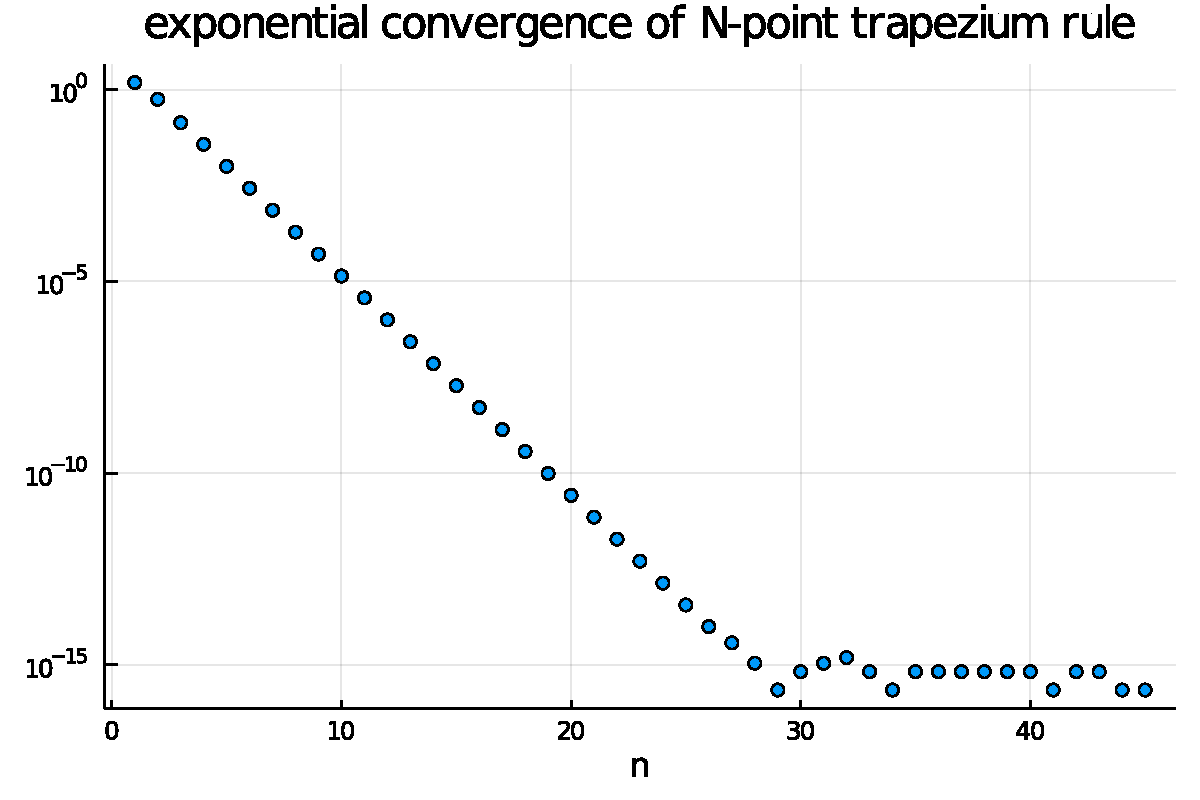
\includegraphics[width=\linewidth]{C:/Users/mfaso/OneDrive/Documents/GitHub/M3M6AppliedComplexAnalysis/output/figures/Lecture6_1_1.pdf}

The accuracy in integration is remarkable as the trapezoidal interpolant does not accurately approximate $f$: we can see clear differences between the functions here:


\begin{lstlisting}
(*@\HLJLn{N}@*)(*@\HLJLoB{=}@*)(*@\HLJLni{20}@*)
(*@\HLJLp{(}@*)(*@\HLJLn{x}@*)(*@\HLJLp{,}@*) (*@\HLJLn{w}@*)(*@\HLJLp{)}@*) (*@\HLJLoB{=}@*) (*@\HLJLnf{periodic{\_}rule}@*)(*@\HLJLp{(}@*)(*@\HLJLn{N}@*)(*@\HLJLp{)}@*)
(*@\HLJLnf{plot}@*)(*@\HLJLp{(}@*)(*@\HLJLnf{Fun}@*)(*@\HLJLp{(}@*)(*@\HLJLn{f}@*)(*@\HLJLp{,}@*) (*@\HLJLni{0}@*) (*@\HLJLoB{..}@*) (*@\HLJLni{2}@*)(*@\HLJLn{\ensuremath{\pi}}@*)(*@\HLJLp{);}@*) (*@\HLJLn{label}@*) (*@\HLJLoB{=}@*) (*@\HLJLs{"{}integrand"{}}@*)(*@\HLJLp{)}@*)
(*@\HLJLnf{plot!}@*)(*@\HLJLp{(}@*)(*@\HLJLn{x}@*)(*@\HLJLp{,}@*) (*@\HLJLn{f}@*)(*@\HLJLoB{.}@*)(*@\HLJLp{(}@*)(*@\HLJLn{x}@*)(*@\HLJLp{);}@*) (*@\HLJLn{label}@*) (*@\HLJLoB{=}@*) (*@\HLJLs{"{}trapezium}@*) (*@\HLJLs{approximation"{}}@*)(*@\HLJLp{)}@*)
\end{lstlisting}

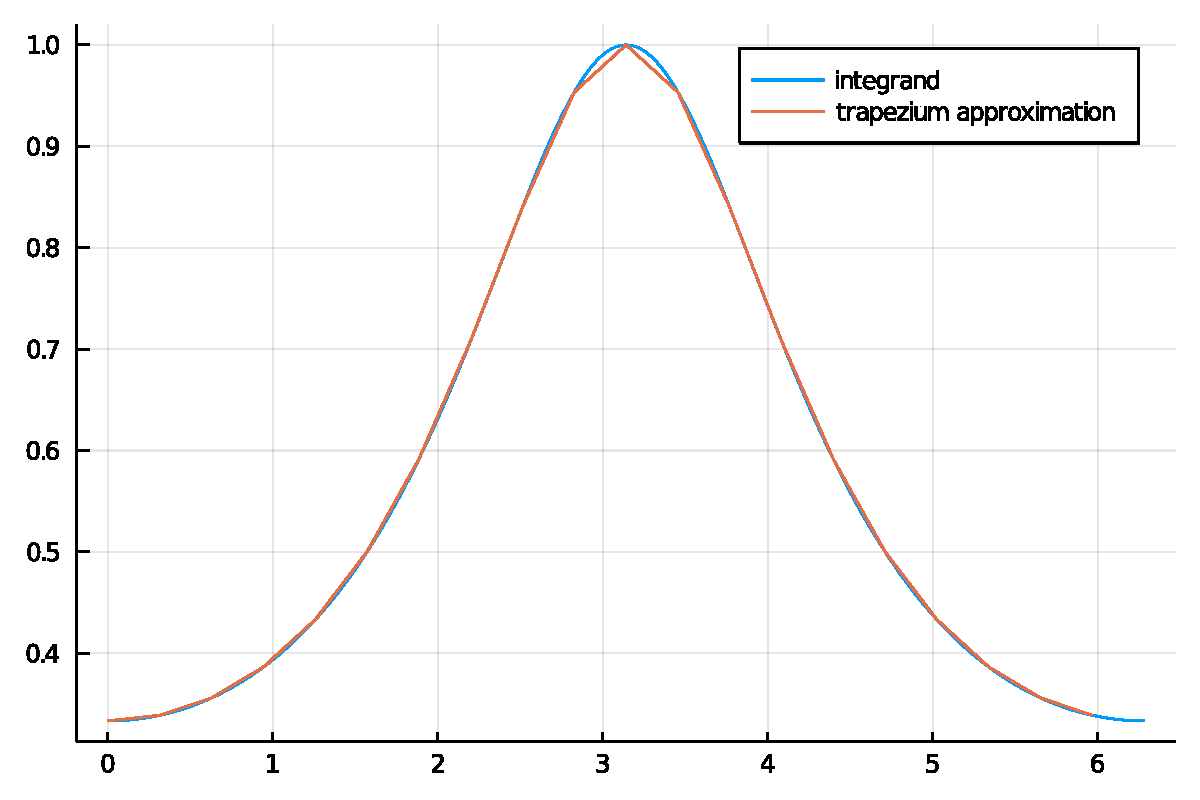
\includegraphics[width=\linewidth]{C:/Users/mfaso/OneDrive/Documents/GitHub/M3M6AppliedComplexAnalysis/output/figures/Lecture6_2_1.pdf}

\subsection{Trapezium rule and Fourier coefficients}
Write

\[
f(\theta) = \sum_{k=-\infty}^\infty \hat f_k \E^{\I k \theta}
\]
and assume that the Fourier coefficients are absolutely summable (true if $f$ is smooth enough):

\[
\sum_{k=-\infty}^\infty |\hat f_k| < \infty.
\]
Note that geometric series tells us that


\begin{align*}
{1 \over 2 \pi} Q_N \E^{\I k \theta} &= {1 \over N} \sum_{j=0}^{N-1} (\E^{2 \pi \I k /N})^j \\
    &= \begin{cases}
        1 & \hbox{if $k = m N$ for some integer $m$} \\
        0 & \hbox{otherwise}
    \end{cases}
\end{align*}
It follows that we can express the Trapezium rule exactly in terms of a sum of Fourier coefficients:


\begin{align*}
{1 \over 2 \pi} Q_N f &= \sum_{k=-\infty}^\infty \hat f_k {1 \over 2 \pi} Q_N \E^{\I k \theta} = \sum_{k=-\infty}^\infty \hat f_k \begin{cases}
        1 & \hbox{if $k = m N$ for some integer $m$} \\
        0 & \hbox{otherwise}
    \end{cases} \\
    &= \cdots + \hat f_{-2N} + \hat f_{-N} + \hat f_0 + \hat f_N + \hat f_{2N} + \cdots
\end{align*}
In other words, the error in the Trapezium rule is bounded by

\[
|\int_0^{2\pi} f(\theta) \D \theta - Q_N f| \leq 2 \pi \sum_{m=1}^\infty \br[|\hat f_{m N}| + |\hat f_{-m N}|]
\]
if we can show fast decay in the coefficients we can prove the observation that trapezium rule converges fast.

\subsection{Decay in Fourier/Laurent coefficients}
Now we consider $g(z)$ such that $g(\E^{\I \theta}) = f(\theta)$, that is, $g$ has the Laurent series

\[
g(z) = \sum_{k=-\infty}^\infty g_k z^k
\]
where $g_k = \hat f_k$. Interestingly, analytic properties of $g$ can be used to show decaying properties in Fourier coefficients of $f$:

\textbf{Theorem (Decay in Fourier/Laurent coefficients)} Suppose $g(z)$ is analytic in a closed annulus $A_{r,R}$ around $0$: $A_r(z_0) = \{z : r \ensuremath{\leq} | z| \ensuremath{\leq} R\}$. Then for all $k$ $|g_k | \leq M\min\left\{{1 \over R^k} , {1 \over r^k}\right\}$ where $M = \sup_{z \in  A_{r,R}} |g(z)|$.

\textbf{Proof} This is a simple application of the ML lemma: let $k \geq 0$, then

\[
|g_k| = {1 \over 2 \pi } \left|\oint_{C_1} {g(\zeta) \over \zeta^{k+1}} \D \zeta\right| = {1 \over 2 \pi}\left|\oint_{C_R} {g(\zeta) \over \zeta^{k+1}} \D \zeta\right| \leq \sup_{\zeta \in C_R} |g(\zeta)| R^{-k} \leq M R^{-k}.
\]
For $k < 0$, we deform the contour to $C_r$. \ensuremath{\blacksquare}

We thus can show fast convergence of Trapezium rule again using geometric series:

\[
\sum_{m=1}^\infty \br[|\hat f_{m N}| + |\hat f_{-m N}|] \leq M \sum_{m=1}^\infty \br[R^{-m N}  + r^{m N}] \leq
M \br[{R^{-N} \over 1 - R^{-N}} + {r^N \over 1 - r^N}].
\]
\emph{Demonstration} The Laurent coefficients of $f(\theta) = {1 \over 2 - \cos \theta}$ satisfies for $k \geq 0$

\[
   |g_k| \leq {2 \over 4 - R -R^{-1}} R^{-k}
\]
for all $R \leq 2 + \sqrt{3}$. The following shows this bound is quite accurate:


\begin{lstlisting}
(*@\HLJLn{g}@*) (*@\HLJLoB{=}@*)(*@\HLJLnf{Fun}@*)(*@\HLJLp{(}@*)(*@\HLJLn{\ensuremath{\theta}}@*) (*@\HLJLoB{->}@*) (*@\HLJLni{1}@*)(*@\HLJLoB{/}@*)(*@\HLJLp{(}@*)(*@\HLJLni{2}@*)(*@\HLJLoB{-}@*)(*@\HLJLnf{cos}@*)(*@\HLJLp{(}@*)(*@\HLJLn{\ensuremath{\theta}}@*)(*@\HLJLp{)),}@*) (*@\HLJLnf{Laurent}@*)(*@\HLJLp{(}@*)(*@\HLJLoB{-}@*)(*@\HLJLn{\ensuremath{\pi}}@*) (*@\HLJLoB{..}@*) (*@\HLJLn{\ensuremath{\pi}}@*)(*@\HLJLp{))}@*)
(*@\HLJLn{g\ensuremath{\_+}}@*) (*@\HLJLoB{=}@*) (*@\HLJLn{g}@*)(*@\HLJLoB{.}@*)(*@\HLJLn{coefficients}@*)(*@\HLJLp{[}@*)(*@\HLJLni{1}@*)(*@\HLJLoB{:}@*)(*@\HLJLni{2}@*)(*@\HLJLoB{:}@*)(*@\HLJLk{end}@*)(*@\HLJLp{]}@*)
(*@\HLJLnf{scatter}@*)(*@\HLJLp{(}@*)(*@\HLJLn{abs}@*)(*@\HLJLoB{.}@*)(*@\HLJLp{(}@*)(*@\HLJLn{g\ensuremath{\_+}}@*)(*@\HLJLp{);}@*) (*@\HLJLn{yscale}@*)(*@\HLJLoB{=:}@*)(*@\HLJLn{log10}@*)(*@\HLJLp{,}@*) (*@\HLJLn{label}@*)(*@\HLJLoB{=}@*)(*@\HLJLs{"{}|g{\_}k|"{}}@*)(*@\HLJLp{,}@*) (*@\HLJLn{legend}@*)(*@\HLJLoB{=:}@*)(*@\HLJLn{bottomleft}@*)(*@\HLJLp{)}@*)
(*@\HLJLn{R}@*) (*@\HLJLoB{=}@*) (*@\HLJLnfB{1.1}@*)
(*@\HLJLnf{scatter!}@*)(*@\HLJLp{(}@*)(*@\HLJLni{2}@*)(*@\HLJLoB{/}@*)(*@\HLJLp{(}@*)(*@\HLJLni{4}@*)(*@\HLJLoB{-}@*)(*@\HLJLn{R}@*)(*@\HLJLoB{-}@*)(*@\HLJLnf{inv}@*)(*@\HLJLp{(}@*)(*@\HLJLn{R}@*)(*@\HLJLp{))}@*)(*@\HLJLoB{*}@*)(*@\HLJLn{R}@*)(*@\HLJLoB{.{\textasciicircum}}@*)(*@\HLJLp{(}@*)(*@\HLJLoB{-}@*)(*@\HLJLp{(}@*)(*@\HLJLni{0}@*)(*@\HLJLoB{:}@*)(*@\HLJLnf{length}@*)(*@\HLJLp{(}@*)(*@\HLJLn{g\ensuremath{\_+}}@*)(*@\HLJLp{))),}@*) (*@\HLJLn{label}@*) (*@\HLJLoB{=}@*) (*@\HLJLs{"{}R}@*) (*@\HLJLs{=}@*) (*@\HLJLsi{{\$}R}@*)(*@\HLJLs{"{}}@*)(*@\HLJLp{)}@*)
(*@\HLJLn{R}@*) (*@\HLJLoB{=}@*) (*@\HLJLnfB{3.5}@*)
(*@\HLJLnf{scatter!}@*)(*@\HLJLp{(}@*)(*@\HLJLni{2}@*)(*@\HLJLoB{/}@*)(*@\HLJLp{(}@*)(*@\HLJLni{4}@*)(*@\HLJLoB{-}@*)(*@\HLJLn{R}@*)(*@\HLJLoB{-}@*)(*@\HLJLnf{inv}@*)(*@\HLJLp{(}@*)(*@\HLJLn{R}@*)(*@\HLJLp{))}@*)(*@\HLJLoB{*}@*)(*@\HLJLn{R}@*)(*@\HLJLoB{.{\textasciicircum}}@*)(*@\HLJLp{(}@*)(*@\HLJLoB{-}@*)(*@\HLJLp{(}@*)(*@\HLJLni{0}@*)(*@\HLJLoB{:}@*)(*@\HLJLnf{length}@*)(*@\HLJLp{(}@*)(*@\HLJLn{g\ensuremath{\_+}}@*)(*@\HLJLp{))),}@*) (*@\HLJLn{label}@*) (*@\HLJLoB{=}@*) (*@\HLJLs{"{}R}@*) (*@\HLJLs{=}@*) (*@\HLJLsi{{\$}R}@*)(*@\HLJLs{"{}}@*)(*@\HLJLp{)}@*)
(*@\HLJLn{R}@*) (*@\HLJLoB{=}@*) (*@\HLJLni{2}@*)(*@\HLJLoB{+}@*)(*@\HLJLnf{sqrt}@*)(*@\HLJLp{(}@*)(*@\HLJLni{3}@*)(*@\HLJLp{)}@*)(*@\HLJLoB{-}@*)(*@\HLJLnfB{0.1}@*)
(*@\HLJLnf{scatter!}@*)(*@\HLJLp{(}@*)(*@\HLJLni{2}@*)(*@\HLJLoB{/}@*)(*@\HLJLp{(}@*)(*@\HLJLni{4}@*)(*@\HLJLoB{-}@*)(*@\HLJLn{R}@*)(*@\HLJLoB{-}@*)(*@\HLJLnf{inv}@*)(*@\HLJLp{(}@*)(*@\HLJLn{R}@*)(*@\HLJLp{))}@*)(*@\HLJLoB{*}@*)(*@\HLJLn{R}@*)(*@\HLJLoB{.{\textasciicircum}}@*)(*@\HLJLp{(}@*)(*@\HLJLoB{-}@*)(*@\HLJLp{(}@*)(*@\HLJLni{0}@*)(*@\HLJLoB{:}@*)(*@\HLJLnf{length}@*)(*@\HLJLp{(}@*)(*@\HLJLn{g\ensuremath{\_+}}@*)(*@\HLJLp{))),}@*) (*@\HLJLn{label}@*) (*@\HLJLoB{=}@*) (*@\HLJLs{"{}R}@*) (*@\HLJLs{=}@*) (*@\HLJLsi{{\$}R}@*)(*@\HLJLs{"{}}@*)(*@\HLJLp{)}@*)
\end{lstlisting}

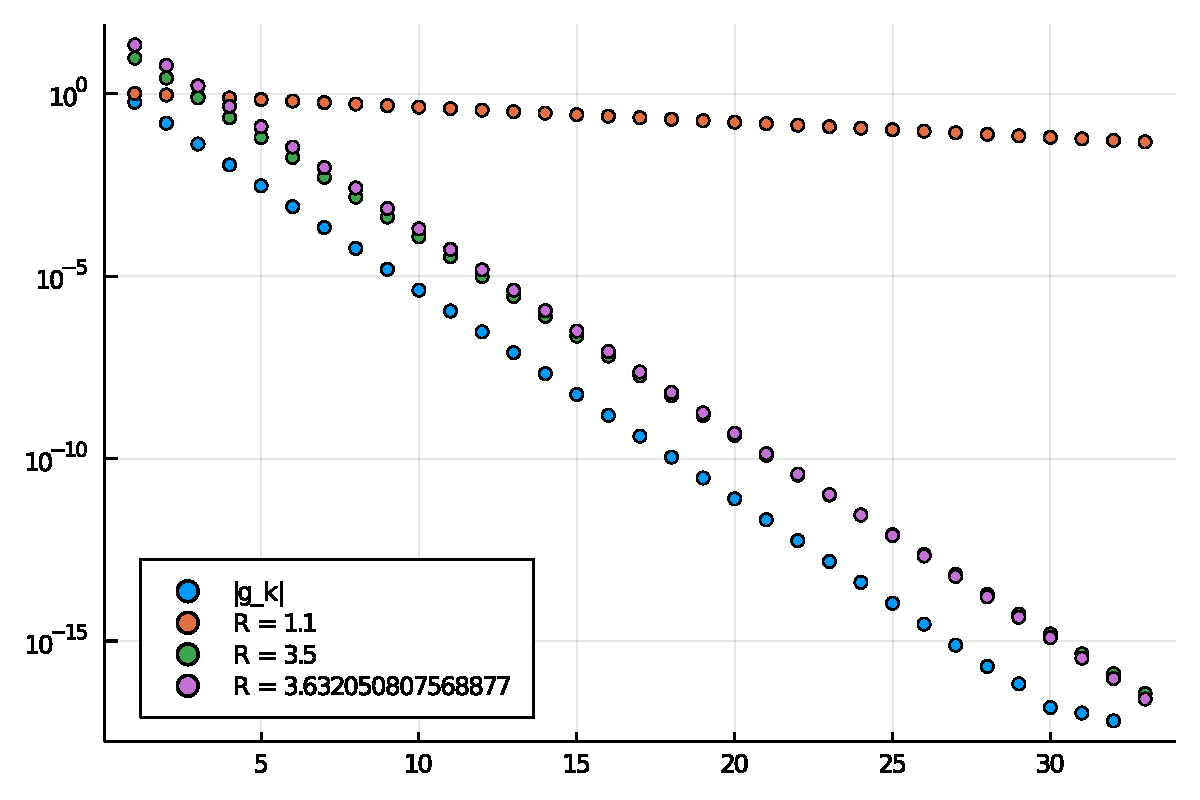
\includegraphics[width=\linewidth]{C:/Users/mfaso/OneDrive/Documents/GitHub/M3M6AppliedComplexAnalysis/output/figures/Lecture6_3_1.pdf}

This fast decay in coefficients explains the fast convergence of the trapezium rule.

\subsection{Complex Trapezium rule}
We can use the map $\gamma$ that defines a closed contour to construct an approximation to integrals over $\gamma$:

\textbf{Definition (Complex trapezium rule)} The \emph{complex trapezium rule} on a contour $\gamma$ (mapped from $[0,2\pi)$) is the approximation

\[
\oint_\gamma f(z) dz \approx  \sum_{j=0}^{N-1} w_j f(z_j)
\]
for

\[
z_j = \gamma(\theta_j) \qquad\hbox{and}\qquad w_j = {2\pi \over N} \gamma'(\theta_j)
\]
\emph{Example (Circle trapezium rule)} On a circle $C_r = \{r \E^{\I \theta} : 0 \leq \theta < 2 \pi\}$, we have

\[
\oint_{C_r} f(z) dz \approx  \sum_{j=0}^{N-1} w_j f(z_j)
\]
for $z_j = r \E^{\I \theta_j}$ and $w_j = {2 \pi \I r \over N}  \E^{\I \theta_j}$.

Here we plot the quadrature points:


\begin{lstlisting}
(*@\HLJLk{function}@*) (*@\HLJLnf{circle{\_}rule}@*)(*@\HLJLp{(}@*)(*@\HLJLn{N}@*)(*@\HLJLp{,}@*) (*@\HLJLn{r}@*)(*@\HLJLp{)}@*)
    (*@\HLJLn{\ensuremath{\theta}}@*) (*@\HLJLoB{=}@*) (*@\HLJLnf{periodic{\_}rule}@*)(*@\HLJLp{(}@*)(*@\HLJLn{N}@*)(*@\HLJLp{)[}@*)(*@\HLJLni{1}@*)(*@\HLJLp{]}@*)
    (*@\HLJLn{r}@*)(*@\HLJLoB{*}@*)(*@\HLJLn{exp}@*)(*@\HLJLoB{.}@*)(*@\HLJLp{(}@*)(*@\HLJLn{im}@*)(*@\HLJLoB{*}@*)(*@\HLJLn{\ensuremath{\theta}}@*)(*@\HLJLp{),}@*) (*@\HLJLni{2}@*)(*@\HLJLn{\ensuremath{\pi}}@*)(*@\HLJLoB{*}@*)(*@\HLJLn{im}@*)(*@\HLJLoB{*}@*)(*@\HLJLn{r}@*)(*@\HLJLoB{/}@*)(*@\HLJLn{N}@*)(*@\HLJLoB{*}@*)(*@\HLJLn{exp}@*)(*@\HLJLoB{.}@*)(*@\HLJLp{(}@*)(*@\HLJLn{im}@*)(*@\HLJLoB{*}@*)(*@\HLJLn{\ensuremath{\theta}}@*)(*@\HLJLp{)}@*)
(*@\HLJLk{end}@*)
(*@\HLJLn{\ensuremath{\zeta}}@*)(*@\HLJLp{,}@*) (*@\HLJLn{w}@*) (*@\HLJLoB{=}@*) (*@\HLJLnf{circle{\_}rule}@*)(*@\HLJLp{(}@*)(*@\HLJLni{20}@*)(*@\HLJLp{,}@*) (*@\HLJLnfB{1.0}@*)(*@\HLJLp{)}@*)
(*@\HLJLnf{scatter}@*)(*@\HLJLp{(}@*)(*@\HLJLn{\ensuremath{\zeta}}@*)(*@\HLJLp{;}@*) (*@\HLJLn{title}@*)(*@\HLJLoB{=}@*)(*@\HLJLs{"{}quadrature}@*) (*@\HLJLs{points"{}}@*)(*@\HLJLp{,}@*) (*@\HLJLn{legend}@*)(*@\HLJLoB{=}@*)(*@\HLJLkc{false}@*)(*@\HLJLp{,}@*) (*@\HLJLn{ratio}@*)(*@\HLJLoB{=}@*)(*@\HLJLnfB{1.0}@*)(*@\HLJLp{)}@*)
\end{lstlisting}

\includegraphics[width=\linewidth]{C:/Users/mfaso/OneDrive/Documents/GitHub/M3M6AppliedComplexAnalysis/output/figures/Lecture6_4_1.pdf}

The Circle trapezium rule is surprisingly accurate for analytic functions, following from the explanation above:


\begin{lstlisting}
(*@\HLJLn{\ensuremath{\zeta}}@*)(*@\HLJLp{,}@*) (*@\HLJLn{w}@*) (*@\HLJLoB{=}@*) (*@\HLJLnf{circle{\_}rule}@*)(*@\HLJLp{(}@*)(*@\HLJLni{20}@*)(*@\HLJLp{,}@*) (*@\HLJLnfB{1.0}@*)(*@\HLJLp{)}@*)
(*@\HLJLn{f}@*) (*@\HLJLoB{=}@*) (*@\HLJLn{z}@*) (*@\HLJLoB{->}@*) (*@\HLJLnf{cos}@*)(*@\HLJLp{(}@*)(*@\HLJLn{z}@*)(*@\HLJLp{)}@*)
(*@\HLJLn{z}@*) (*@\HLJLoB{=}@*) (*@\HLJLnfB{0.1}@*)(*@\HLJLoB{+}@*)(*@\HLJLnfB{0.2}@*)(*@\HLJLn{im}@*)
(*@\HLJLnf{sum}@*)(*@\HLJLp{(}@*)(*@\HLJLn{f}@*)(*@\HLJLoB{.}@*)(*@\HLJLp{(}@*)(*@\HLJLn{\ensuremath{\zeta}}@*)(*@\HLJLp{)}@*)(*@\HLJLoB{./}@*)(*@\HLJLp{(}@*)(*@\HLJLn{\ensuremath{\zeta}}@*) (*@\HLJLoB{.-}@*) (*@\HLJLn{z}@*)(*@\HLJLp{)}@*)(*@\HLJLoB{.*}@*)(*@\HLJLn{w}@*)(*@\HLJLp{)}@*)(*@\HLJLoB{/}@*)(*@\HLJLp{(}@*)(*@\HLJLni{2}@*)(*@\HLJLn{\ensuremath{\pi}}@*)(*@\HLJLoB{*}@*)(*@\HLJLn{im}@*)(*@\HLJLp{)}@*) (*@\HLJLoB{-}@*) (*@\HLJLnf{f}@*)(*@\HLJLp{(}@*)(*@\HLJLn{z}@*)(*@\HLJLp{)}@*)
\end{lstlisting}

\begin{lstlisting}
-9.814371537686384e-14 - 1.3076345561913172e-14im
\end{lstlisting}


\subsection{Application: Numerical differentiation}
Calculating high-order derivatives using limits is numerically unstable. Here is a demonstration using finite-differences: making $h$ small does not increase the accuracy after a certain point:


\begin{lstlisting}
(*@\HLJLk{using}@*) (*@\HLJLn{SpecialFunctions}@*)
(*@\HLJLn{f}@*) (*@\HLJLoB{=}@*) (*@\HLJLn{z}@*) (*@\HLJLoB{->}@*) (*@\HLJLnf{gamma}@*)(*@\HLJLp{(}@*)(*@\HLJLn{z}@*)(*@\HLJLp{)}@*)
(*@\HLJLn{fp}@*) (*@\HLJLoB{=}@*) (*@\HLJLn{z}@*) (*@\HLJLoB{->}@*) (*@\HLJLnf{gamma}@*)(*@\HLJLp{(}@*)(*@\HLJLn{z}@*)(*@\HLJLp{)}@*)(*@\HLJLnf{polygamma}@*)(*@\HLJLp{(}@*)(*@\HLJLni{0}@*)(*@\HLJLp{,}@*)(*@\HLJLn{z}@*)(*@\HLJLp{)}@*) (*@\HLJLcs{{\#}}@*) (*@\HLJLcs{exact}@*) (*@\HLJLcs{derivative}@*)
(*@\HLJLn{x}@*) (*@\HLJLoB{=}@*) (*@\HLJLnfB{1.2}@*)
(*@\HLJLn{fp{\_}fd}@*) (*@\HLJLoB{=}@*) (*@\HLJLp{[(}@*)(*@\HLJLn{h}@*)(*@\HLJLoB{=}@*)(*@\HLJLnfB{2.0}@*)(*@\HLJLoB{{\textasciicircum}}@*)(*@\HLJLp{(}@*)(*@\HLJLoB{-}@*)(*@\HLJLn{n}@*)(*@\HLJLp{);}@*)  (*@\HLJLp{(}@*)(*@\HLJLnf{f}@*)(*@\HLJLp{(}@*)(*@\HLJLn{x}@*)(*@\HLJLoB{+}@*)(*@\HLJLn{h}@*)(*@\HLJLp{)}@*)(*@\HLJLoB{-}@*)(*@\HLJLnf{f}@*)(*@\HLJLp{(}@*)(*@\HLJLn{x}@*)(*@\HLJLp{))}@*)(*@\HLJLoB{/}@*)(*@\HLJLn{h}@*)(*@\HLJLp{)}@*) (*@\HLJLk{for}@*) (*@\HLJLn{n}@*) (*@\HLJLoB{=}@*) (*@\HLJLni{1}@*)(*@\HLJLoB{:}@*)(*@\HLJLni{50}@*)(*@\HLJLp{]}@*)
(*@\HLJLnf{scatter}@*)(*@\HLJLp{(}@*)(*@\HLJLn{abs}@*)(*@\HLJLoB{.}@*)(*@\HLJLp{(}@*)(*@\HLJLn{fp{\_}fd}@*) (*@\HLJLoB{.-}@*) (*@\HLJLnf{fp}@*)(*@\HLJLp{(}@*)(*@\HLJLn{x}@*)(*@\HLJLp{));}@*) (*@\HLJLn{yscale}@*)(*@\HLJLoB{=:}@*)(*@\HLJLn{log10}@*)(*@\HLJLp{,}@*) (*@\HLJLn{legend}@*)(*@\HLJLoB{=}@*)(*@\HLJLkc{false}@*)(*@\HLJLp{,}@*) (*@\HLJLn{title}@*) (*@\HLJLoB{=}@*) (*@\HLJLs{"{}error}@*) (*@\HLJLs{of}@*) (*@\HLJLs{finite-difference}@*) (*@\HLJLs{with}@*) (*@\HLJLs{h=2{\textasciicircum}(-n)"{}}@*)(*@\HLJLp{,}@*) (*@\HLJLn{xlabel}@*)(*@\HLJLoB{=}@*)(*@\HLJLs{"{}n"{}}@*)(*@\HLJLp{)}@*)
\end{lstlisting}

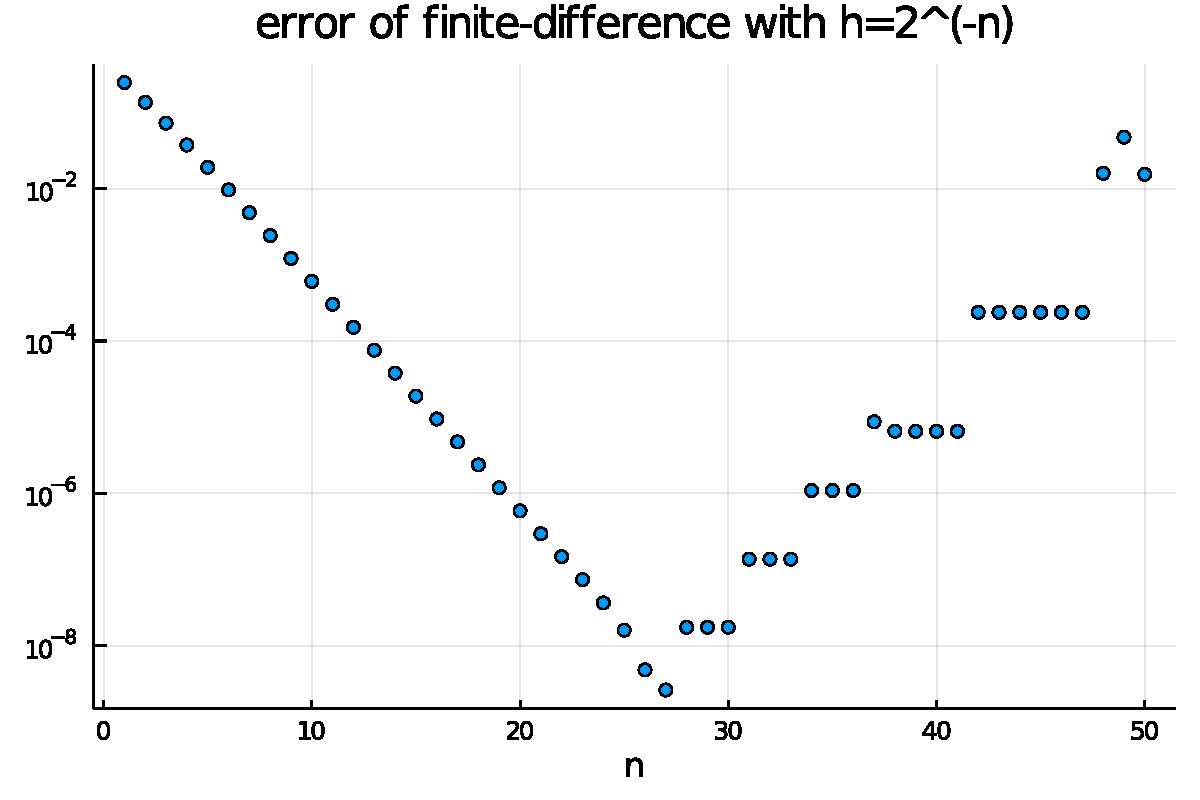
\includegraphics[width=\linewidth]{C:/Users/mfaso/OneDrive/Documents/GitHub/M3M6AppliedComplexAnalysis/output/figures/Lecture6_6_1.pdf}

But the Cauchy integral formula for derivatives tells us that we can reduce a derivative to a contour integral, which can be computed stably:


\begin{lstlisting}
(*@\HLJLn{trap{\_}fp}@*) (*@\HLJLoB{=}@*) (*@\HLJLp{[((}@*)(*@\HLJLn{\ensuremath{\zeta}}@*)(*@\HLJLp{,}@*) (*@\HLJLn{w}@*)(*@\HLJLp{)}@*) (*@\HLJLoB{=}@*) (*@\HLJLnf{circle{\_}rule}@*)(*@\HLJLp{(}@*)(*@\HLJLn{n}@*)(*@\HLJLp{,}@*) (*@\HLJLnfB{0.5}@*)(*@\HLJLp{);}@*)
        (*@\HLJLn{\ensuremath{\zeta}}@*) (*@\HLJLoB{.+=}@*) (*@\HLJLn{x}@*)(*@\HLJLp{;}@*) (*@\HLJLcs{{\#}}@*) (*@\HLJLcs{circle}@*) (*@\HLJLcs{around}@*) (*@\HLJLcs{x}@*)
       (*@\HLJLnf{sum}@*)(*@\HLJLp{(}@*)(*@\HLJLn{f}@*)(*@\HLJLoB{.}@*)(*@\HLJLp{(}@*)(*@\HLJLn{\ensuremath{\zeta}}@*)(*@\HLJLp{)}@*)(*@\HLJLoB{./}@*)(*@\HLJLp{(}@*)(*@\HLJLn{\ensuremath{\zeta}}@*) (*@\HLJLoB{.-}@*) (*@\HLJLn{x}@*)(*@\HLJLp{)}@*)(*@\HLJLoB{.{\textasciicircum}}@*)(*@\HLJLni{2}@*) (*@\HLJLoB{.*}@*)(*@\HLJLn{w}@*)(*@\HLJLp{)}@*)(*@\HLJLoB{/}@*)(*@\HLJLp{(}@*)(*@\HLJLni{2}@*)(*@\HLJLn{\ensuremath{\pi}}@*)(*@\HLJLoB{*}@*)(*@\HLJLn{im}@*)(*@\HLJLp{))}@*) (*@\HLJLk{for}@*) (*@\HLJLn{n}@*)(*@\HLJLoB{=}@*)(*@\HLJLni{1}@*)(*@\HLJLoB{:}@*)(*@\HLJLni{50}@*)(*@\HLJLp{]}@*)

(*@\HLJLnf{scatter}@*)(*@\HLJLp{(}@*)(*@\HLJLn{abs}@*)(*@\HLJLoB{.}@*)(*@\HLJLp{(}@*)(*@\HLJLn{trap{\_}fp}@*) (*@\HLJLoB{.-}@*) (*@\HLJLn{fp}@*)(*@\HLJLoB{.}@*)(*@\HLJLp{(}@*)(*@\HLJLn{x}@*)(*@\HLJLp{));}@*) (*@\HLJLn{yscale}@*)(*@\HLJLoB{=:}@*)(*@\HLJLn{log10}@*)(*@\HLJLp{,}@*)
       (*@\HLJLn{title}@*)(*@\HLJLoB{=}@*)(*@\HLJLs{"{}Error}@*) (*@\HLJLs{of}@*) (*@\HLJLs{trapezium}@*) (*@\HLJLs{rule}@*) (*@\HLJLs{applied}@*) (*@\HLJLs{to}@*) (*@\HLJLs{Cauchy}@*) (*@\HLJLs{integral}@*) (*@\HLJLs{formula"{}}@*)(*@\HLJLp{,}@*) (*@\HLJLn{xlabel}@*)(*@\HLJLoB{=}@*)(*@\HLJLs{"{}n"{}}@*)(*@\HLJLp{,}@*) (*@\HLJLn{legend}@*)(*@\HLJLoB{=}@*)(*@\HLJLkc{false}@*)(*@\HLJLp{)}@*)
\end{lstlisting}

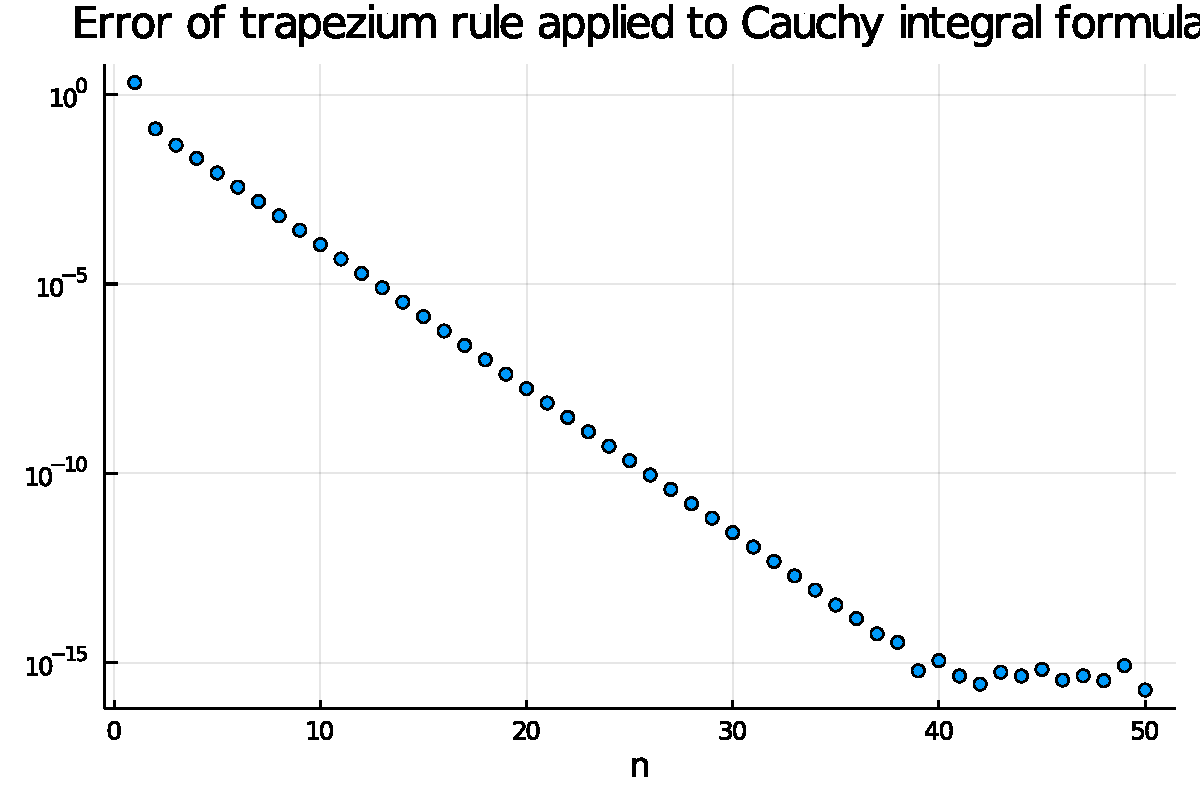
\includegraphics[width=\linewidth]{C:/Users/mfaso/OneDrive/Documents/GitHub/M3M6AppliedComplexAnalysis/output/figures/Lecture6_7_1.pdf}

The exponential convergence of the complex trapezium rule is a consequence of $f(\gamma(t))$ being 2\ensuremath{\pi}-periodic:


\begin{lstlisting}
(*@\HLJLn{\ensuremath{\theta}}@*) (*@\HLJLoB{=}@*) (*@\HLJLnf{periodic{\_}rule}@*)(*@\HLJLp{(}@*)(*@\HLJLni{100}@*)(*@\HLJLp{)[}@*)(*@\HLJLni{1}@*)(*@\HLJLp{]}@*)
(*@\HLJLn{\ensuremath{\zeta}}@*) (*@\HLJLoB{=}@*) (*@\HLJLn{x}@*) (*@\HLJLoB{.+}@*) (*@\HLJLnfB{0.5}@*)(*@\HLJLoB{*}@*)(*@\HLJLn{exp}@*)(*@\HLJLoB{.}@*)(*@\HLJLp{(}@*)(*@\HLJLn{im}@*)(*@\HLJLoB{*}@*)(*@\HLJLn{\ensuremath{\theta}}@*)(*@\HLJLp{)}@*)
(*@\HLJLnf{plot}@*)(*@\HLJLp{(}@*)(*@\HLJLn{\ensuremath{\theta}}@*)(*@\HLJLp{,}@*) (*@\HLJLn{real}@*)(*@\HLJLoB{.}@*)(*@\HLJLp{(}@*)(*@\HLJLn{f}@*)(*@\HLJLoB{.}@*)(*@\HLJLp{(}@*)(*@\HLJLn{\ensuremath{\zeta}}@*)(*@\HLJLp{));}@*)(*@\HLJLn{label}@*)(*@\HLJLoB{=}@*)(*@\HLJLs{"{}real(f)"{}}@*)(*@\HLJLp{)}@*)
(*@\HLJLnf{plot!}@*)(*@\HLJLp{(}@*)(*@\HLJLn{\ensuremath{\theta}}@*)(*@\HLJLp{,}@*)(*@\HLJLn{imag}@*)(*@\HLJLoB{.}@*)(*@\HLJLp{(}@*)(*@\HLJLn{f}@*)(*@\HLJLoB{.}@*)(*@\HLJLp{(}@*)(*@\HLJLn{\ensuremath{\zeta}}@*)(*@\HLJLp{));}@*)(*@\HLJLn{label}@*)(*@\HLJLoB{=}@*)(*@\HLJLs{"{}imag(f)"{}}@*)(*@\HLJLp{)}@*)
\end{lstlisting}

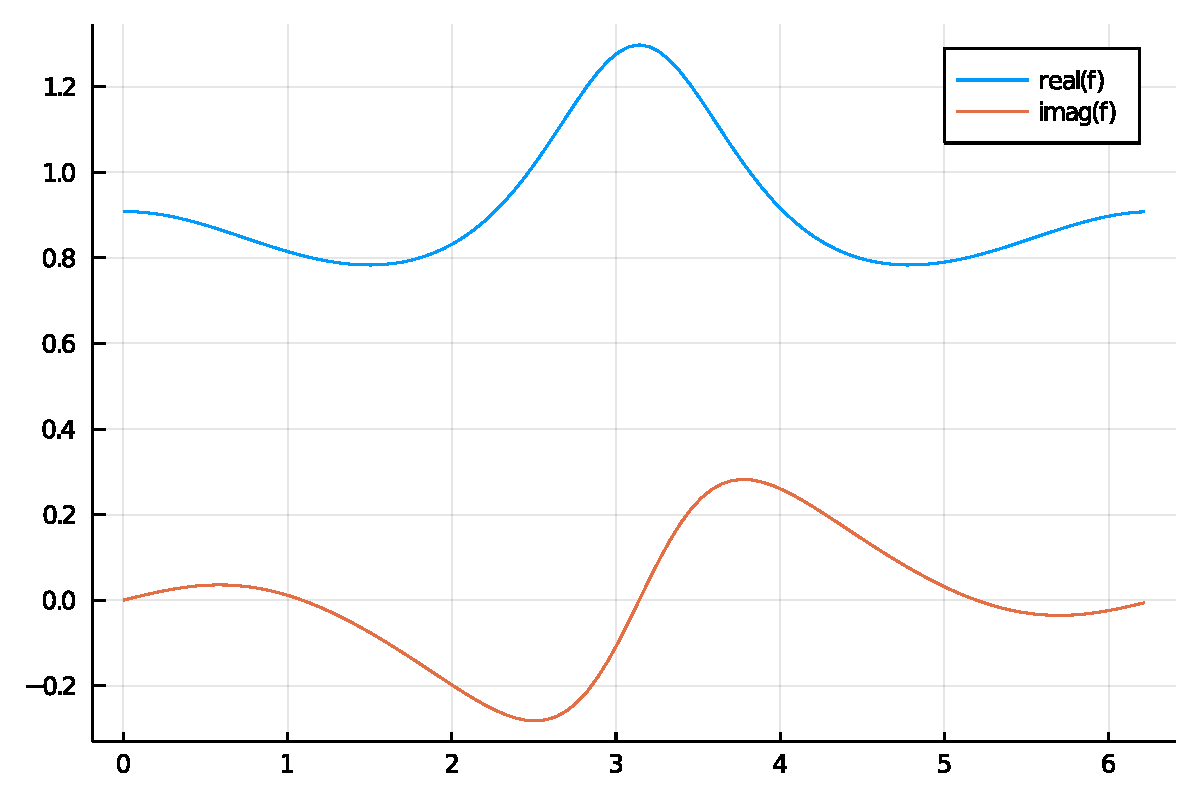
\includegraphics[width=\linewidth]{C:/Users/mfaso/OneDrive/Documents/GitHub/M3M6AppliedComplexAnalysis/output/figures/Lecture6_8_1.pdf}

Therefore, the integrand of Cauchy's integral formula is periodic and analytic (if $f$ is analytic) on the circular contour.

We can take things further and use this to calculate higher order derivatives, with some care taken for choosing the radius:


\begin{lstlisting}
(*@\HLJLn{k}@*)(*@\HLJLoB{=}@*)(*@\HLJLni{100}@*)
(*@\HLJLn{r}@*) (*@\HLJLoB{=}@*) (*@\HLJLnfB{1.0}@*)(*@\HLJLn{k}@*)
(*@\HLJLn{g}@*) (*@\HLJLoB{=}@*) (*@\HLJLnf{Fun}@*)(*@\HLJLp{(}@*) (*@\HLJLn{\ensuremath{\zeta}}@*) (*@\HLJLoB{->}@*) (*@\HLJLnf{exp}@*)(*@\HLJLp{(}@*)(*@\HLJLn{\ensuremath{\zeta}}@*)(*@\HLJLp{)}@*)(*@\HLJLoB{/}@*)(*@\HLJLp{(}@*)(*@\HLJLn{\ensuremath{\zeta}}@*) (*@\HLJLoB{-}@*) (*@\HLJLnfB{0.1}@*)(*@\HLJLp{)}@*)(*@\HLJLoB{{\textasciicircum}}@*)(*@\HLJLp{(}@*)(*@\HLJLn{k}@*)(*@\HLJLoB{+}@*)(*@\HLJLni{1}@*)(*@\HLJLp{),}@*) (*@\HLJLnf{Circle}@*)(*@\HLJLp{(}@*)(*@\HLJLnfB{0.1}@*)(*@\HLJLp{,}@*)(*@\HLJLn{r}@*)(*@\HLJLp{))}@*)
(*@\HLJLnf{factorial}@*)(*@\HLJLp{(}@*)(*@\HLJLnfB{1.0}@*)(*@\HLJLn{k}@*)(*@\HLJLp{)}@*)(*@\HLJLoB{/}@*)(*@\HLJLp{(}@*)(*@\HLJLni{2}@*)(*@\HLJLn{\ensuremath{\pi}}@*)(*@\HLJLoB{*}@*)(*@\HLJLn{im}@*)(*@\HLJLp{)}@*) (*@\HLJLoB{*}@*) (*@\HLJLnf{sum}@*)(*@\HLJLp{(}@*)(*@\HLJLn{g}@*)(*@\HLJLp{)}@*) (*@\HLJLoB{-}@*) (*@\HLJLnf{exp}@*)(*@\HLJLp{(}@*)(*@\HLJLnfB{0.1}@*)(*@\HLJLp{)}@*)
\end{lstlisting}

\begin{lstlisting}
-7.993605777301127e-15 + 3.675487826103639e-16im
\end{lstlisting}


\href{https://www-m3.ma.tum.de/foswiki/pub/M3/Allgemeines/FolkmarBornemannPublications/FoCM_Stability_Cauchy_Integrals.pdf}{Bornemann 2011} investigates this further and optimizes the radius.

\emph{Example (Ellipse trapezium rule)} On an ellipse $\{a \cos \theta + b \I \sin \theta : 0 \leq \theta < 2 \pi\}$ we have

\[
\oint_\gamma f(z) dz \approx  \sum_{j=0}^{N-1} w_j f(z_j)
\]
for $z_j = a \cos \theta_j + b \I \sin \theta_j$ and $w_j = {2 \pi \over N} (-a \sin \theta_j + \I b \cos \theta_j)$.

We can use the ellipse trapezium rule in place of the circle trapezium rule and still achieve accurate results. This gives us flexibility in avoiding singularities. Consider

\[
f(z) = 1/(25z^2 + 1)
\]
which has poles at $\pm  \I/5$. Using an ellipse allows us to design a contour that avoids these singularities:


\begin{lstlisting}
(*@\HLJLnf{scatter}@*)(*@\HLJLp{([}@*)(*@\HLJLni{1}@*)(*@\HLJLoB{/}@*)(*@\HLJLni{5}@*)(*@\HLJLn{im}@*)(*@\HLJLp{,}@*)(*@\HLJLoB{-}@*)(*@\HLJLni{1}@*)(*@\HLJLoB{/}@*)(*@\HLJLni{5}@*)(*@\HLJLn{im}@*)(*@\HLJLp{];}@*) (*@\HLJLn{label}@*)(*@\HLJLoB{=}@*)(*@\HLJLs{"{}singularities"{}}@*)(*@\HLJLp{)}@*)
(*@\HLJLn{\ensuremath{\theta}}@*) (*@\HLJLoB{=}@*) (*@\HLJLnf{range}@*)(*@\HLJLp{(}@*)(*@\HLJLni{0}@*)(*@\HLJLp{;}@*) (*@\HLJLn{stop}@*)(*@\HLJLoB{=}@*)(*@\HLJLni{2}@*)(*@\HLJLn{\ensuremath{\pi}}@*)(*@\HLJLp{,}@*) (*@\HLJLn{length}@*)(*@\HLJLoB{=}@*)(*@\HLJLni{2000}@*)(*@\HLJLp{)}@*)
(*@\HLJLn{a}@*) (*@\HLJLoB{=}@*) (*@\HLJLni{2}@*)(*@\HLJLp{;}@*) (*@\HLJLn{b}@*)(*@\HLJLoB{=}@*) (*@\HLJLnfB{0.1}@*)
(*@\HLJLnf{plot!}@*)(*@\HLJLp{(}@*)(*@\HLJLn{a}@*) (*@\HLJLoB{*}@*) (*@\HLJLn{cos}@*)(*@\HLJLoB{.}@*)(*@\HLJLp{(}@*)(*@\HLJLn{\ensuremath{\theta}}@*)(*@\HLJLp{)}@*) (*@\HLJLoB{+}@*) (*@\HLJLn{im}@*)(*@\HLJLoB{*}@*)(*@\HLJLn{b}@*) (*@\HLJLoB{*}@*) (*@\HLJLn{sin}@*)(*@\HLJLoB{.}@*)(*@\HLJLp{(}@*)(*@\HLJLn{\ensuremath{\theta}}@*)(*@\HLJLp{);}@*) (*@\HLJLn{label}@*)(*@\HLJLoB{=}@*)(*@\HLJLs{"{}ellipse"{}}@*)(*@\HLJLp{,}@*) (*@\HLJLn{ratio}@*) (*@\HLJLoB{=}@*) (*@\HLJLnfB{1.0}@*)(*@\HLJLp{)}@*)
\end{lstlisting}

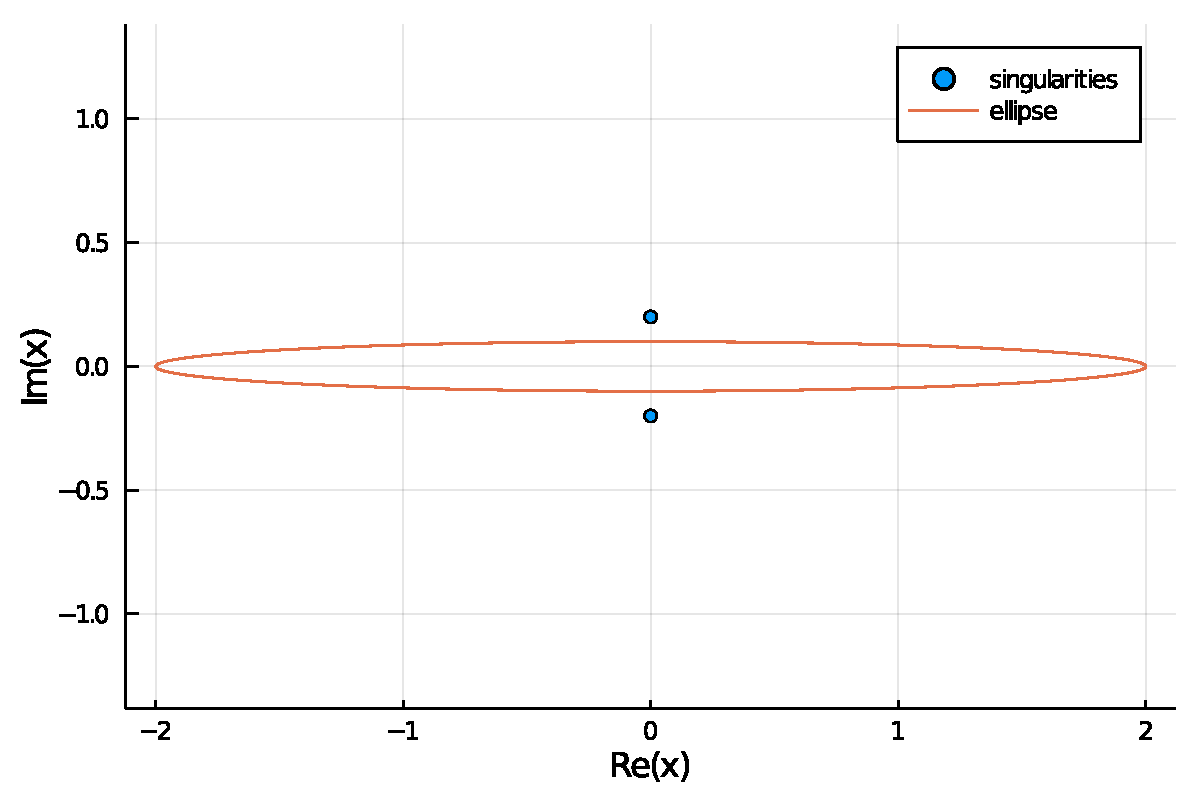
\includegraphics[width=\linewidth]{C:/Users/mfaso/OneDrive/Documents/GitHub/M3M6AppliedComplexAnalysis/output/figures/Lecture6_10_1.pdf}

Thus we can still use Cauchy's integral formula:


\begin{lstlisting}
(*@\HLJLn{x}@*) (*@\HLJLoB{=}@*) (*@\HLJLnfB{0.1}@*)
(*@\HLJLn{f}@*) (*@\HLJLoB{=}@*) (*@\HLJLn{z}@*) (*@\HLJLoB{->}@*) (*@\HLJLni{1}@*)(*@\HLJLoB{/}@*)(*@\HLJLp{(}@*)(*@\HLJLni{25}@*)(*@\HLJLn{z}@*)(*@\HLJLoB{{\textasciicircum}}@*)(*@\HLJLni{2}@*) (*@\HLJLoB{+}@*) (*@\HLJLni{1}@*)(*@\HLJLp{)}@*)
(*@\HLJLk{function}@*) (*@\HLJLnf{ellipse{\_}rule}@*)(*@\HLJLp{(}@*)(*@\HLJLn{n}@*)(*@\HLJLp{,}@*) (*@\HLJLn{a}@*)(*@\HLJLp{,}@*) (*@\HLJLn{b}@*)(*@\HLJLp{)}@*)
    (*@\HLJLn{\ensuremath{\theta}}@*) (*@\HLJLoB{=}@*) (*@\HLJLnf{periodic{\_}rule}@*)(*@\HLJLp{(}@*)(*@\HLJLn{n}@*)(*@\HLJLp{)[}@*)(*@\HLJLni{1}@*)(*@\HLJLp{]}@*)
    (*@\HLJLn{a}@*)(*@\HLJLoB{*}@*)(*@\HLJLn{cos}@*)(*@\HLJLoB{.}@*)(*@\HLJLp{(}@*)(*@\HLJLn{\ensuremath{\theta}}@*)(*@\HLJLp{)}@*) (*@\HLJLoB{+}@*) (*@\HLJLn{b}@*)(*@\HLJLoB{*}@*)(*@\HLJLn{im}@*)(*@\HLJLoB{*}@*)(*@\HLJLn{sin}@*)(*@\HLJLoB{.}@*)(*@\HLJLp{(}@*)(*@\HLJLn{\ensuremath{\theta}}@*)(*@\HLJLp{),}@*) (*@\HLJLni{2}@*)(*@\HLJLn{\ensuremath{\pi}}@*)(*@\HLJLoB{/}@*)(*@\HLJLn{n}@*)(*@\HLJLoB{*}@*)(*@\HLJLp{(}@*)(*@\HLJLoB{-}@*)(*@\HLJLn{a}@*)(*@\HLJLoB{*}@*)(*@\HLJLn{sin}@*)(*@\HLJLoB{.}@*)(*@\HLJLp{(}@*)(*@\HLJLn{\ensuremath{\theta}}@*)(*@\HLJLp{)}@*) (*@\HLJLoB{+}@*) (*@\HLJLn{im}@*)(*@\HLJLoB{*}@*)(*@\HLJLn{b}@*)(*@\HLJLoB{*}@*)(*@\HLJLn{cos}@*)(*@\HLJLoB{.}@*)(*@\HLJLp{(}@*)(*@\HLJLn{\ensuremath{\theta}}@*)(*@\HLJLp{))}@*)
(*@\HLJLk{end}@*)
(*@\HLJLn{f{\_}ellipse}@*) (*@\HLJLoB{=}@*) (*@\HLJLp{[((}@*)(*@\HLJLn{z}@*)(*@\HLJLp{,}@*) (*@\HLJLn{w}@*)(*@\HLJLp{)}@*) (*@\HLJLoB{=}@*) (*@\HLJLnf{ellipse{\_}rule}@*)(*@\HLJLp{(}@*)(*@\HLJLn{n}@*)(*@\HLJLp{,}@*) (*@\HLJLn{a}@*)(*@\HLJLp{,}@*) (*@\HLJLn{b}@*)(*@\HLJLp{);}@*) (*@\HLJLnf{sum}@*)(*@\HLJLp{(}@*)(*@\HLJLn{f}@*)(*@\HLJLoB{.}@*)(*@\HLJLp{(}@*)(*@\HLJLn{z}@*)(*@\HLJLp{)}@*)(*@\HLJLoB{./}@*)(*@\HLJLp{(}@*)(*@\HLJLn{z}@*)(*@\HLJLoB{.-}@*)(*@\HLJLn{x}@*)(*@\HLJLp{)}@*)(*@\HLJLoB{.*}@*)(*@\HLJLn{w}@*)(*@\HLJLp{)}@*)(*@\HLJLoB{/}@*)(*@\HLJLp{(}@*)(*@\HLJLni{2}@*)(*@\HLJLn{\ensuremath{\pi}}@*)(*@\HLJLoB{*}@*)(*@\HLJLn{im}@*)(*@\HLJLp{))}@*) (*@\HLJLk{for}@*) (*@\HLJLn{n}@*)(*@\HLJLoB{=}@*)(*@\HLJLni{1}@*)(*@\HLJLoB{:}@*)(*@\HLJLni{1000}@*)(*@\HLJLp{]}@*)
(*@\HLJLnf{plot}@*)(*@\HLJLp{(}@*)(*@\HLJLn{abs}@*)(*@\HLJLoB{.}@*)(*@\HLJLp{(}@*)(*@\HLJLn{f{\_}ellipse}@*) (*@\HLJLoB{.-}@*) (*@\HLJLnf{f}@*)(*@\HLJLp{(}@*)(*@\HLJLn{x}@*)(*@\HLJLp{));}@*) (*@\HLJLn{yscale}@*)(*@\HLJLoB{=:}@*)(*@\HLJLn{log10}@*)(*@\HLJLp{,}@*) (*@\HLJLn{title}@*)(*@\HLJLoB{=}@*)(*@\HLJLs{"{}convergence}@*) (*@\HLJLs{of}@*) (*@\HLJLs{n-point}@*) (*@\HLJLs{ellipse}@*) (*@\HLJLs{approximation"{}}@*)(*@\HLJLp{,}@*) (*@\HLJLn{legend}@*)(*@\HLJLoB{=}@*)(*@\HLJLkc{false}@*)(*@\HLJLp{,}@*) (*@\HLJLn{xlabel}@*)(*@\HLJLoB{=}@*)(*@\HLJLs{"{}n"{}}@*)(*@\HLJLp{)}@*)
\end{lstlisting}

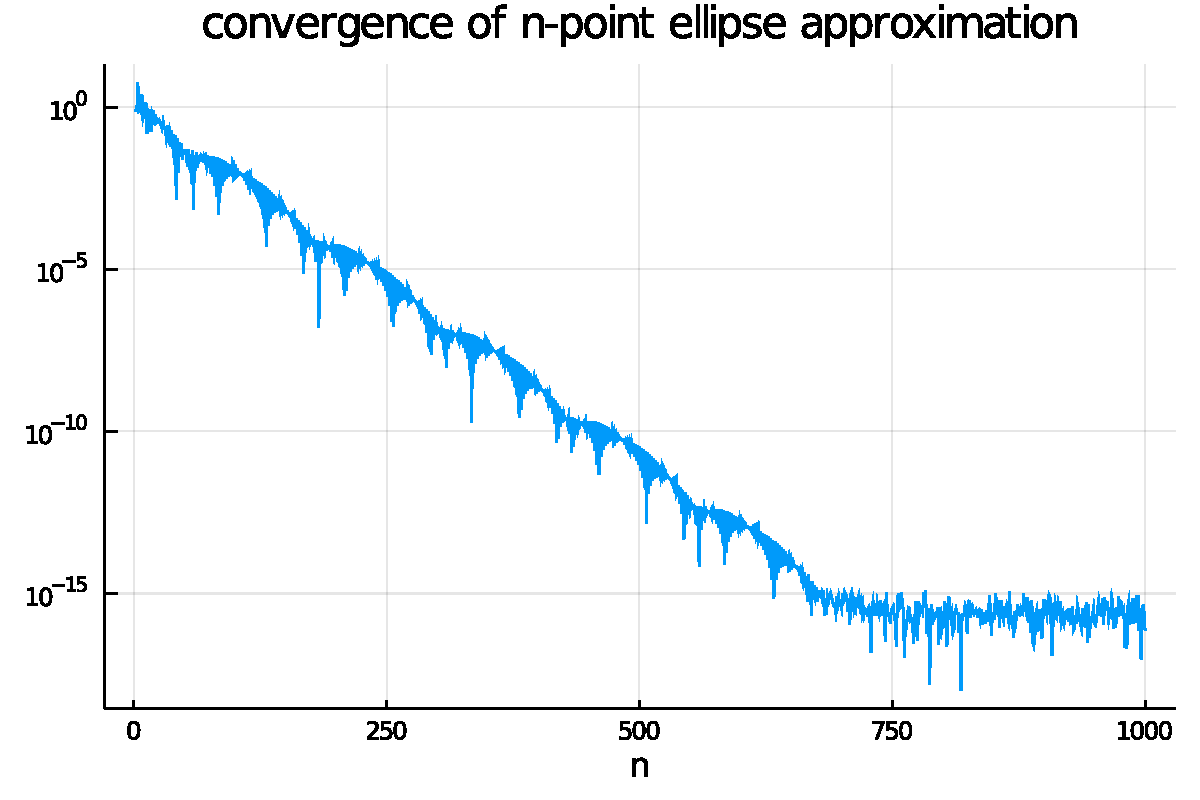
\includegraphics[width=\linewidth]{C:/Users/mfaso/OneDrive/Documents/GitHub/M3M6AppliedComplexAnalysis/output/figures/Lecture6_11_1.pdf}

\subsection{Taylor series versus Cauchy integral formula}
The Taylor series gives a polynomial approximation to $f$. The Cauchy's integral formula discretisation gives a rational approximation, which is more adaptable and does not require knowing the derivatives of $f$:


\begin{lstlisting}
(*@\HLJLk{using}@*) (*@\HLJLn{ComplexPhasePortrait}@*)
(*@\HLJLn{f}@*) (*@\HLJLoB{=}@*) (*@\HLJLn{z}@*) (*@\HLJLoB{->}@*) (*@\HLJLnf{sqrt}@*)(*@\HLJLp{(}@*)(*@\HLJLn{z}@*)(*@\HLJLp{)}@*)
(*@\HLJLk{function}@*) (*@\HLJLnf{sqrt{\_}n}@*)(*@\HLJLp{(}@*)(*@\HLJLn{n}@*)(*@\HLJLp{,}@*)(*@\HLJLn{z}@*)(*@\HLJLp{,}@*)(*@\HLJLn{z\ensuremath{\_0}}@*)(*@\HLJLp{)}@*)
    (*@\HLJLn{ret}@*) (*@\HLJLoB{=}@*) (*@\HLJLnf{sqrt}@*)(*@\HLJLp{(}@*)(*@\HLJLn{z\ensuremath{\_0}}@*)(*@\HLJLp{)}@*)
    (*@\HLJLn{c}@*) (*@\HLJLoB{=}@*) (*@\HLJLnfB{0.5}@*)(*@\HLJLoB{/}@*)(*@\HLJLn{ret}@*)(*@\HLJLoB{*}@*)(*@\HLJLp{(}@*)(*@\HLJLn{z}@*)(*@\HLJLoB{-}@*)(*@\HLJLn{z\ensuremath{\_0}}@*)(*@\HLJLp{)}@*)
    (*@\HLJLk{for}@*) (*@\HLJLn{k}@*)(*@\HLJLoB{=}@*)(*@\HLJLni{1}@*)(*@\HLJLoB{:}@*)(*@\HLJLn{n}@*)
        (*@\HLJLn{ret}@*) (*@\HLJLoB{+=}@*) (*@\HLJLn{c}@*)
        (*@\HLJLn{c}@*) (*@\HLJLoB{*=}@*) (*@\HLJLoB{-}@*)(*@\HLJLp{(}@*)(*@\HLJLni{2}@*)(*@\HLJLn{k}@*)(*@\HLJLoB{-}@*)(*@\HLJLni{1}@*)(*@\HLJLp{)}@*)(*@\HLJLoB{/}@*)(*@\HLJLp{(}@*)(*@\HLJLni{2}@*)(*@\HLJLoB{*}@*)(*@\HLJLp{(}@*)(*@\HLJLn{k}@*)(*@\HLJLoB{+}@*)(*@\HLJLni{1}@*)(*@\HLJLp{)}@*)(*@\HLJLoB{*}@*)(*@\HLJLn{z\ensuremath{\_0}}@*)(*@\HLJLp{)}@*)(*@\HLJLoB{*}@*)(*@\HLJLp{(}@*)(*@\HLJLn{z}@*)(*@\HLJLoB{-}@*)(*@\HLJLn{z\ensuremath{\_0}}@*)(*@\HLJLp{)}@*)
    (*@\HLJLk{end}@*)
    (*@\HLJLn{ret}@*)
(*@\HLJLk{end}@*)
(*@\HLJLn{z\ensuremath{\_0}}@*) (*@\HLJLoB{=}@*) (*@\HLJLnfB{0.3}@*)
(*@\HLJLn{n}@*) (*@\HLJLoB{=}@*) (*@\HLJLni{40}@*)
(*@\HLJLnf{phaseplot}@*)(*@\HLJLp{(}@*)(*@\HLJLoB{-}@*)(*@\HLJLnfB{2..2}@*)(*@\HLJLp{,}@*) (*@\HLJLoB{-}@*)(*@\HLJLnfB{2..2}@*)(*@\HLJLp{,}@*) (*@\HLJLn{z}@*) (*@\HLJLoB{->}@*) (*@\HLJLn{sqrt{\_}n}@*)(*@\HLJLoB{.}@*)(*@\HLJLp{(}@*)(*@\HLJLn{n}@*)(*@\HLJLp{,}@*)(*@\HLJLn{z}@*)(*@\HLJLp{,}@*)(*@\HLJLn{z\ensuremath{\_0}}@*)(*@\HLJLp{))}@*)
\end{lstlisting}

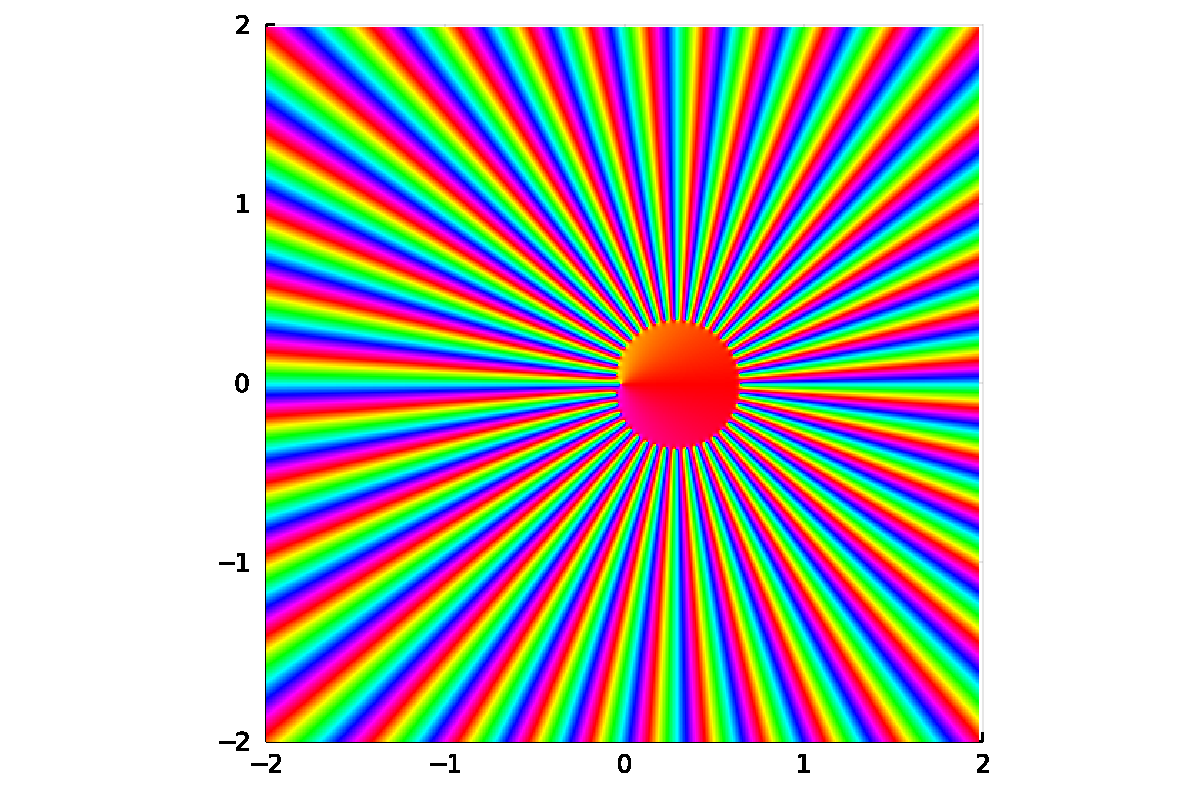
\includegraphics[width=\linewidth]{C:/Users/mfaso/OneDrive/Documents/GitHub/M3M6AppliedComplexAnalysis/output/figures/Lecture6_12_1.pdf}

Here we see that the approximation is valid on the expected ellipse:


\begin{lstlisting}
(*@\HLJLp{(}@*)(*@\HLJLn{\ensuremath{\zeta}}@*)(*@\HLJLp{,}@*) (*@\HLJLn{w}@*)(*@\HLJLp{)}@*) (*@\HLJLoB{=}@*) (*@\HLJLnf{ellipse{\_}rule}@*)(*@\HLJLp{(}@*)(*@\HLJLni{20}@*)(*@\HLJLp{,}@*) (*@\HLJLnfB{0.28}@*)(*@\HLJLp{,}@*) (*@\HLJLnfB{1.0}@*)(*@\HLJLp{);}@*)
(*@\HLJLn{\ensuremath{\zeta}}@*)  (*@\HLJLoB{.=}@*) (*@\HLJLn{\ensuremath{\zeta}}@*) (*@\HLJLoB{.+}@*) (*@\HLJLnfB{0.3}@*)(*@\HLJLp{;}@*)
(*@\HLJLn{f{\_}c}@*) (*@\HLJLoB{=}@*) (*@\HLJLn{z}@*) (*@\HLJLoB{->}@*)  (*@\HLJLnf{sum}@*)(*@\HLJLp{(}@*)(*@\HLJLn{f}@*)(*@\HLJLoB{.}@*)(*@\HLJLp{(}@*)(*@\HLJLn{\ensuremath{\zeta}}@*)(*@\HLJLp{)}@*)(*@\HLJLoB{./}@*)(*@\HLJLp{(}@*)(*@\HLJLn{\ensuremath{\zeta}}@*)(*@\HLJLoB{.-}@*)(*@\HLJLn{z}@*)(*@\HLJLp{)}@*)(*@\HLJLoB{.*}@*)(*@\HLJLn{w}@*)(*@\HLJLp{)}@*)(*@\HLJLoB{/}@*)(*@\HLJLp{(}@*)(*@\HLJLni{2}@*)(*@\HLJLn{\ensuremath{\pi}}@*)(*@\HLJLoB{*}@*)(*@\HLJLn{im}@*)(*@\HLJLp{)}@*)
(*@\HLJLnf{phaseplot}@*)(*@\HLJLp{(}@*)(*@\HLJLoB{-}@*)(*@\HLJLnfB{2..2}@*)(*@\HLJLp{,}@*) (*@\HLJLoB{-}@*)(*@\HLJLni{2}@*) (*@\HLJLoB{..}@*) (*@\HLJLni{2}@*)(*@\HLJLp{,}@*) (*@\HLJLn{f{\_}c}@*)(*@\HLJLp{)}@*)
\end{lstlisting}

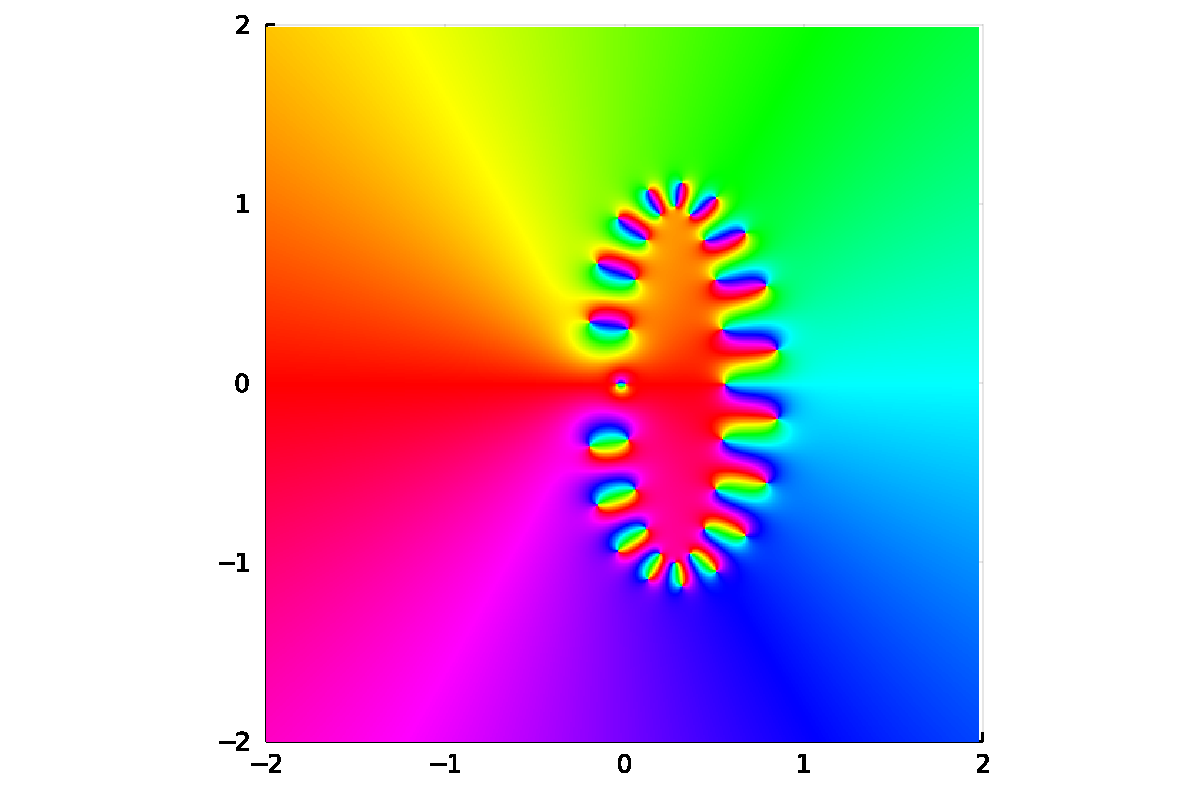
\includegraphics[width=\linewidth]{C:/Users/mfaso/OneDrive/Documents/GitHub/M3M6AppliedComplexAnalysis/output/figures/Lecture6_13_1.pdf}

\begin{lstlisting}
(*@\HLJLp{(}@*)(*@\HLJLn{\ensuremath{\zeta}}@*)(*@\HLJLp{,}@*) (*@\HLJLn{w}@*)(*@\HLJLp{)}@*) (*@\HLJLoB{=}@*) (*@\HLJLnf{ellipse{\_}rule}@*)(*@\HLJLp{(}@*)(*@\HLJLni{1000}@*)(*@\HLJLp{,}@*) (*@\HLJLnfB{0.28}@*)(*@\HLJLp{,}@*) (*@\HLJLnfB{1.0}@*)(*@\HLJLp{);}@*)
(*@\HLJLn{\ensuremath{\zeta}}@*)  (*@\HLJLoB{.=}@*) (*@\HLJLn{\ensuremath{\zeta}}@*) (*@\HLJLoB{.+}@*) (*@\HLJLnfB{0.3}@*)(*@\HLJLp{;}@*)
(*@\HLJLn{f{\_}c}@*) (*@\HLJLoB{=}@*) (*@\HLJLn{z}@*) (*@\HLJLoB{->}@*)  (*@\HLJLnf{sum}@*)(*@\HLJLp{(}@*)(*@\HLJLn{f}@*)(*@\HLJLoB{.}@*)(*@\HLJLp{(}@*)(*@\HLJLn{\ensuremath{\zeta}}@*)(*@\HLJLp{)}@*)(*@\HLJLoB{./}@*)(*@\HLJLp{(}@*)(*@\HLJLn{\ensuremath{\zeta}}@*)(*@\HLJLoB{.-}@*)(*@\HLJLn{z}@*)(*@\HLJLp{)}@*)(*@\HLJLoB{.*}@*)(*@\HLJLn{w}@*)(*@\HLJLp{)}@*)(*@\HLJLoB{/}@*)(*@\HLJLp{(}@*)(*@\HLJLni{2}@*)(*@\HLJLn{\ensuremath{\pi}}@*)(*@\HLJLoB{*}@*)(*@\HLJLn{im}@*)(*@\HLJLp{)}@*)
(*@\HLJLnf{f{\_}c}@*)(*@\HLJLp{(}@*)(*@\HLJLnfB{0.5}@*)(*@\HLJLp{)}@*) (*@\HLJLoB{-}@*) (*@\HLJLnf{sqrt}@*)(*@\HLJLp{(}@*)(*@\HLJLnfB{0.5}@*)(*@\HLJLp{)}@*)
\end{lstlisting}

\begin{lstlisting}
-3.907985046680551e-14 - 2.9403565414571575e-17im
\end{lstlisting}



\end{document}
